\chapter{Exécution pratique du CAS}

\begin{center}
    \makebox[\textwidth]{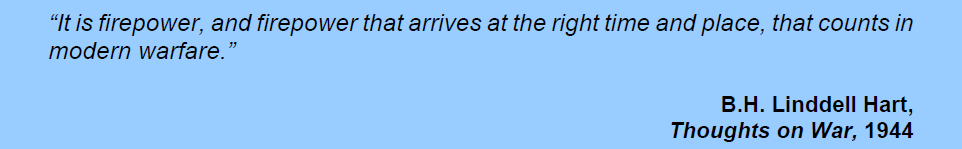
\includegraphics[width=\paperwidth]{quote5.png}}
\end{center}

\e
    \item Déroulement d'une mission \gls{cas}:
    \begin{figure}[H]
        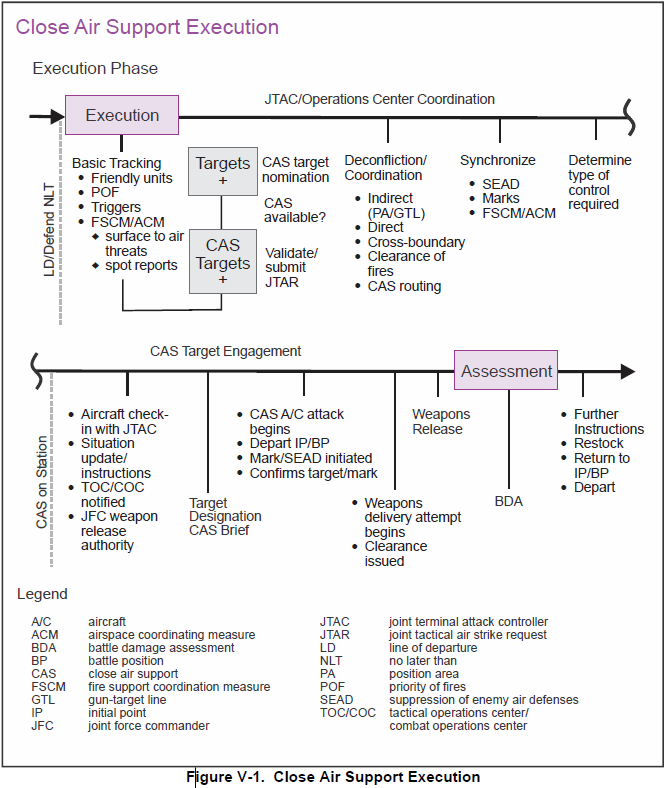
\includegraphics[width=\textwidth]{execution-full.png}
        \caption{Déroulement d'une mission.}
        \label{fig:casflow-full}
    \end{figure}
    \item Cas flow simplifié:
    \begin{figure}[H]
        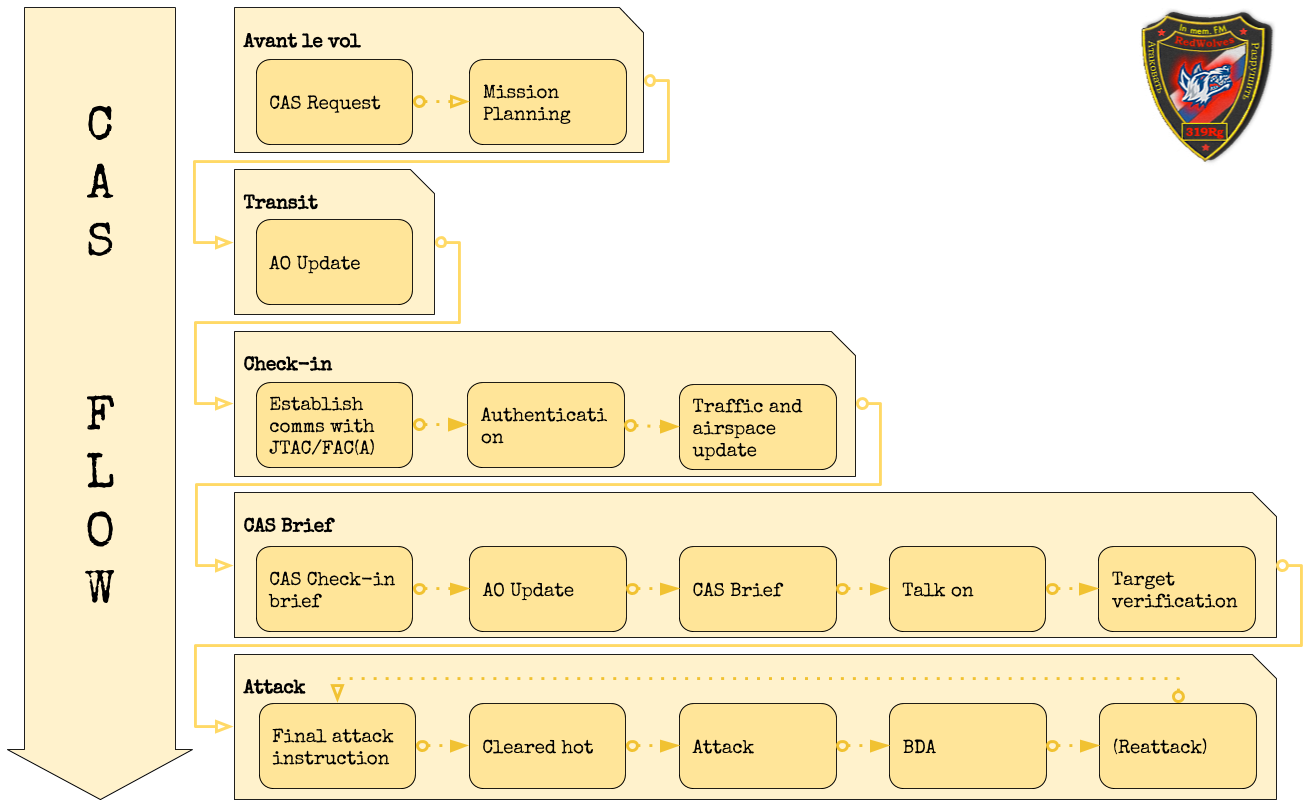
\includegraphics[width=\textwidth]{CASFlow.png}
        \caption{Cas flow simplifié.}
        \label{fig:casflow}
    \end{figure}
\ed

\e
    \item
    Ce chapitre présente le déroulement pratique d’une mission \acrshort{cas}. Le template qui y est présenté illustre une mission \acrshort{cas} typique, et fournit un guide pour le \acrshort{jtac}/\acrshort{faca} et le pilote pour les aider à remplir leur mission.
    \item Le déroulement présenté ici commence après le décollage, et se termine lorsque la patrouille de \acrshort{cas} est sur le retour.
\ed

\section{Routing}
\e
    \item Le routing consiste à diriger les appareils d’un point à un autre.
    \item Extrait du \jp:\\
    \begin{figure}[H]
        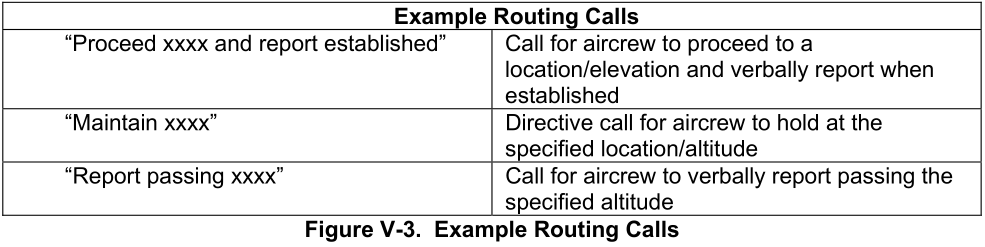
\includegraphics[width=\textwidth]{routing.png}
        \caption{Routing.}
        \label{fig:routing}
    \end{figure}
    \item Exemples:\\
    \ee
        \item Routing standard, demande de maintien de position:\\
        \begin{figure}[H]
            
\includegraphics[width=\textwidth]{routing_ex1.png}
            \caption{Routing: maintien de position.}
            \label{fig:routingpos}
        \end{figure}
        \item Si le contrôleur n'est pas certain de la position et de l'altitude de l'appareil, il doit demander les informations:\\
        \begin{figure}[H]
            
\includegraphics[width=\textwidth]{routing_ex2.png}
            \caption{Routing: demande d'information.}
            \label{fig:routinginfo}
        \end{figure}
        \item Ordre de se diriger vers un point:\\
        \begin{figure}[H]
            
\includegraphics[width=\textwidth]{routing_ex3.png}
            \caption{Routing: ordre.}
            \label{fig:routingorder}
        \end{figure}
        \item Information relative à une menace:\\
        \begin{figure}[H]
            
\includegraphics[width=\textwidth]{routing_ex4.png}
            \caption{Routing: information menace.}
            \label{fig:routingthreat}
        \end{figure}
        \item Information relative aux activités alliées:\\
        \begin{figure}[H]
            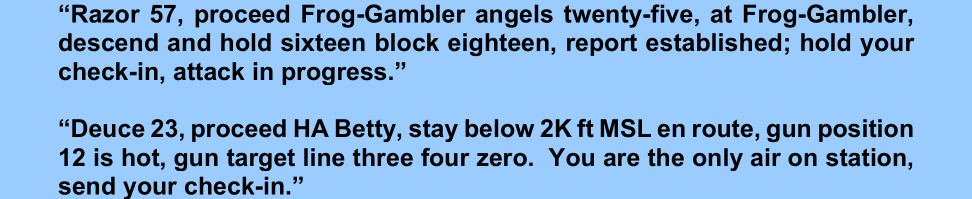
\includegraphics[width=\textwidth]{routing_ex5.png}
            \caption{Routing: information alliés.}
            \label{fig:routingallies}
        \end{figure}
    \ed
\ed

\section{Check-in}

\e
    \item
    Le check-in est la première phase du \acrshort{cas} en tant que tel. C’est l’appel effectué de l’appareil en \acrshort{cas} vers le \acrshort{jtac}/\acrshort{faca} pour lui signifier qu’il est prêt à remplir sa mission de \acrshort{cas}.
    \item Comme le check-in peut prendre un certain temps, un appel préliminaire devrait être effectué. Par exemple:
\ed

\begin{lstlisting}[caption=Appel préliminaire, label=preliminary_call]
    PIRATE, ici REDWOLF, pour check-in, quand dispo.
\end{lstlisting}

\re
    \item Format du check-in:
    \begin{figure}[H]
        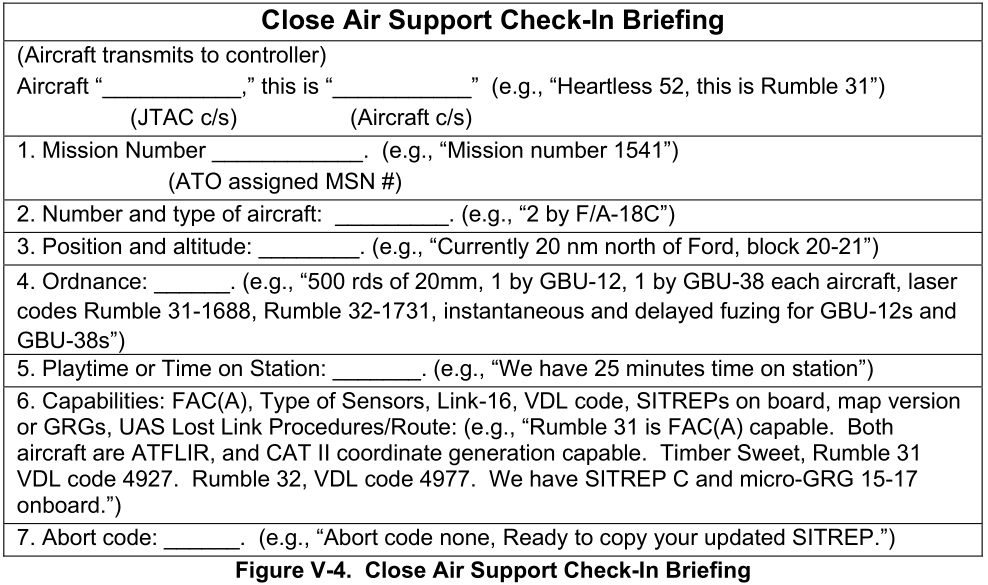
\includegraphics[width=\textwidth]{checkin.png}
        \caption{Format check-in.}
        \label{fig:checkin}
    \end{figure}
    \item S'il le souhaite, le \acrshort{jtac}/\acrshort{faca} peut demander un check-in abrégé:
    \begin{figure}[H]
        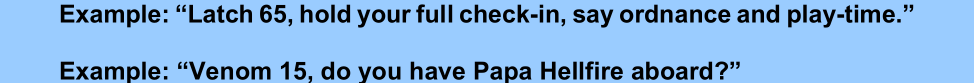
\includegraphics[width=\textwidth]{abbregcheckin.png}
        \caption{Format check-in abrégé.}
        \label{fig:abbregcheckin}
    \end{figure}
\ed
